\chapter{Barrier Forming: Separating Polygonal Sets with Minimum Sets of Lines}\label{ch:bf}
\thispagestyle{myheadings}

After two chapters' discussion on covering perimeters or regions, which is essentially separating 
some critical polygonal regions from the outside workspace. 
This chapter digs deeper into this problem by studying the separation of more than two regions. 
To simplify the problem, a line-of-sight sensing model will be adopted, where each sensor can cover
an unobstructed line segment like a laser beam. Also, the regions are assumed to be polygonal.

The objective in this case is to minimize the number of sensors used to separate these polygonal sets 
at the existence of obstacles.
% The main objective here is to minimize the number of sensor used.
The problem is NP-hard even for the problem of separating two sets of regions with the minimum number of lines. 
Still, integer programming can provide a near-optimal solution for around 20 objects in a reasonable amount of time. 

\section{Introduction}
Consider the scenario where one or more rogue agents (e.g., criminals) may be hiding in several isolated regions in a 2D workspace. To prevent them from potentially escaping from these regions to other nearby vulnerable regions, we may wish to set up line-of-sight sensors to detect if rogue agents attempt to escape. For the setup, a natural question one may ask is: what is the minimum number of line segments that are needed to form the desired barrier? The same setting finds many other practical applications, for example, for the identical setting, we may use the deployed sensors to track the movement of agents between different set of regions, e.g., understanding the flow of people between residential areas to commercial areas, which can benefit large-scale decision making, e.g., to help properly allocating resources for improving the city infrastructure. 
%
Alternatively, the computed line segments can serve as patrolling routes for autonomous agents (robots or humans) for actively monitoring intrusions, where the agents can always keep tracking events along the segments for which they are responsible.

%Barrier forming \cite{}, i.e. separating multiple sets of objects from each other,
%where each set may contain multiple scattered objects mix among other object sets, finds many real-world applications,
%e.g., erecting security fences around buildings,
%isolating different groups of agents (e.g., people, animals), 
%designing routes for patrolling robots to detect invaders, and so on. 
%multi-agent search for rouge agents, and so on. 
%These applications shares the common objective of better coverage or sensing of the environment with guards. 
%In reality, the types of barriers varies from barriers with range sensibility like lidar, visibility-based barriers like cameras or guards, to physical straight line fences or walls.
%
Motivated by the above-stated scenarios and inspired by earlier research in robotics on barrier forming \cite{kloder2007barrier,kloder2008partial}, i.e., erecting barriers for separating regions of interest, in this chapter, we examine the variation of finding the minimum number of straight line segments for isolating multiple sets of points of polygons in a two-dimensional workspace. 
Fig~\ref{fig:bf-ex}[left] illustrates an instance where three colored polygonal sets are to be separated from each other and the grey polygons are obstacles. Fig~\ref{fig:surf-ex}[right] shows a possible solution which is fairly non-trivial 
to obtain. 
%
%The problem finds applications in many practical scenarios where geometric separation is needed, for example, the deployment of a minimum set of  line-of-sight security beams to guard critical areas from intrusions. 
%dividing different rooms in a floor or buildings from each other to prevent the %spread of virus or contagious diseases,
%designing the surveillance routes for guards that walk on a straight route,
%building fences for regions among different security level that are not allowed 
%to have connections, and so on. 

\begin{figure}[t]
    \centering
    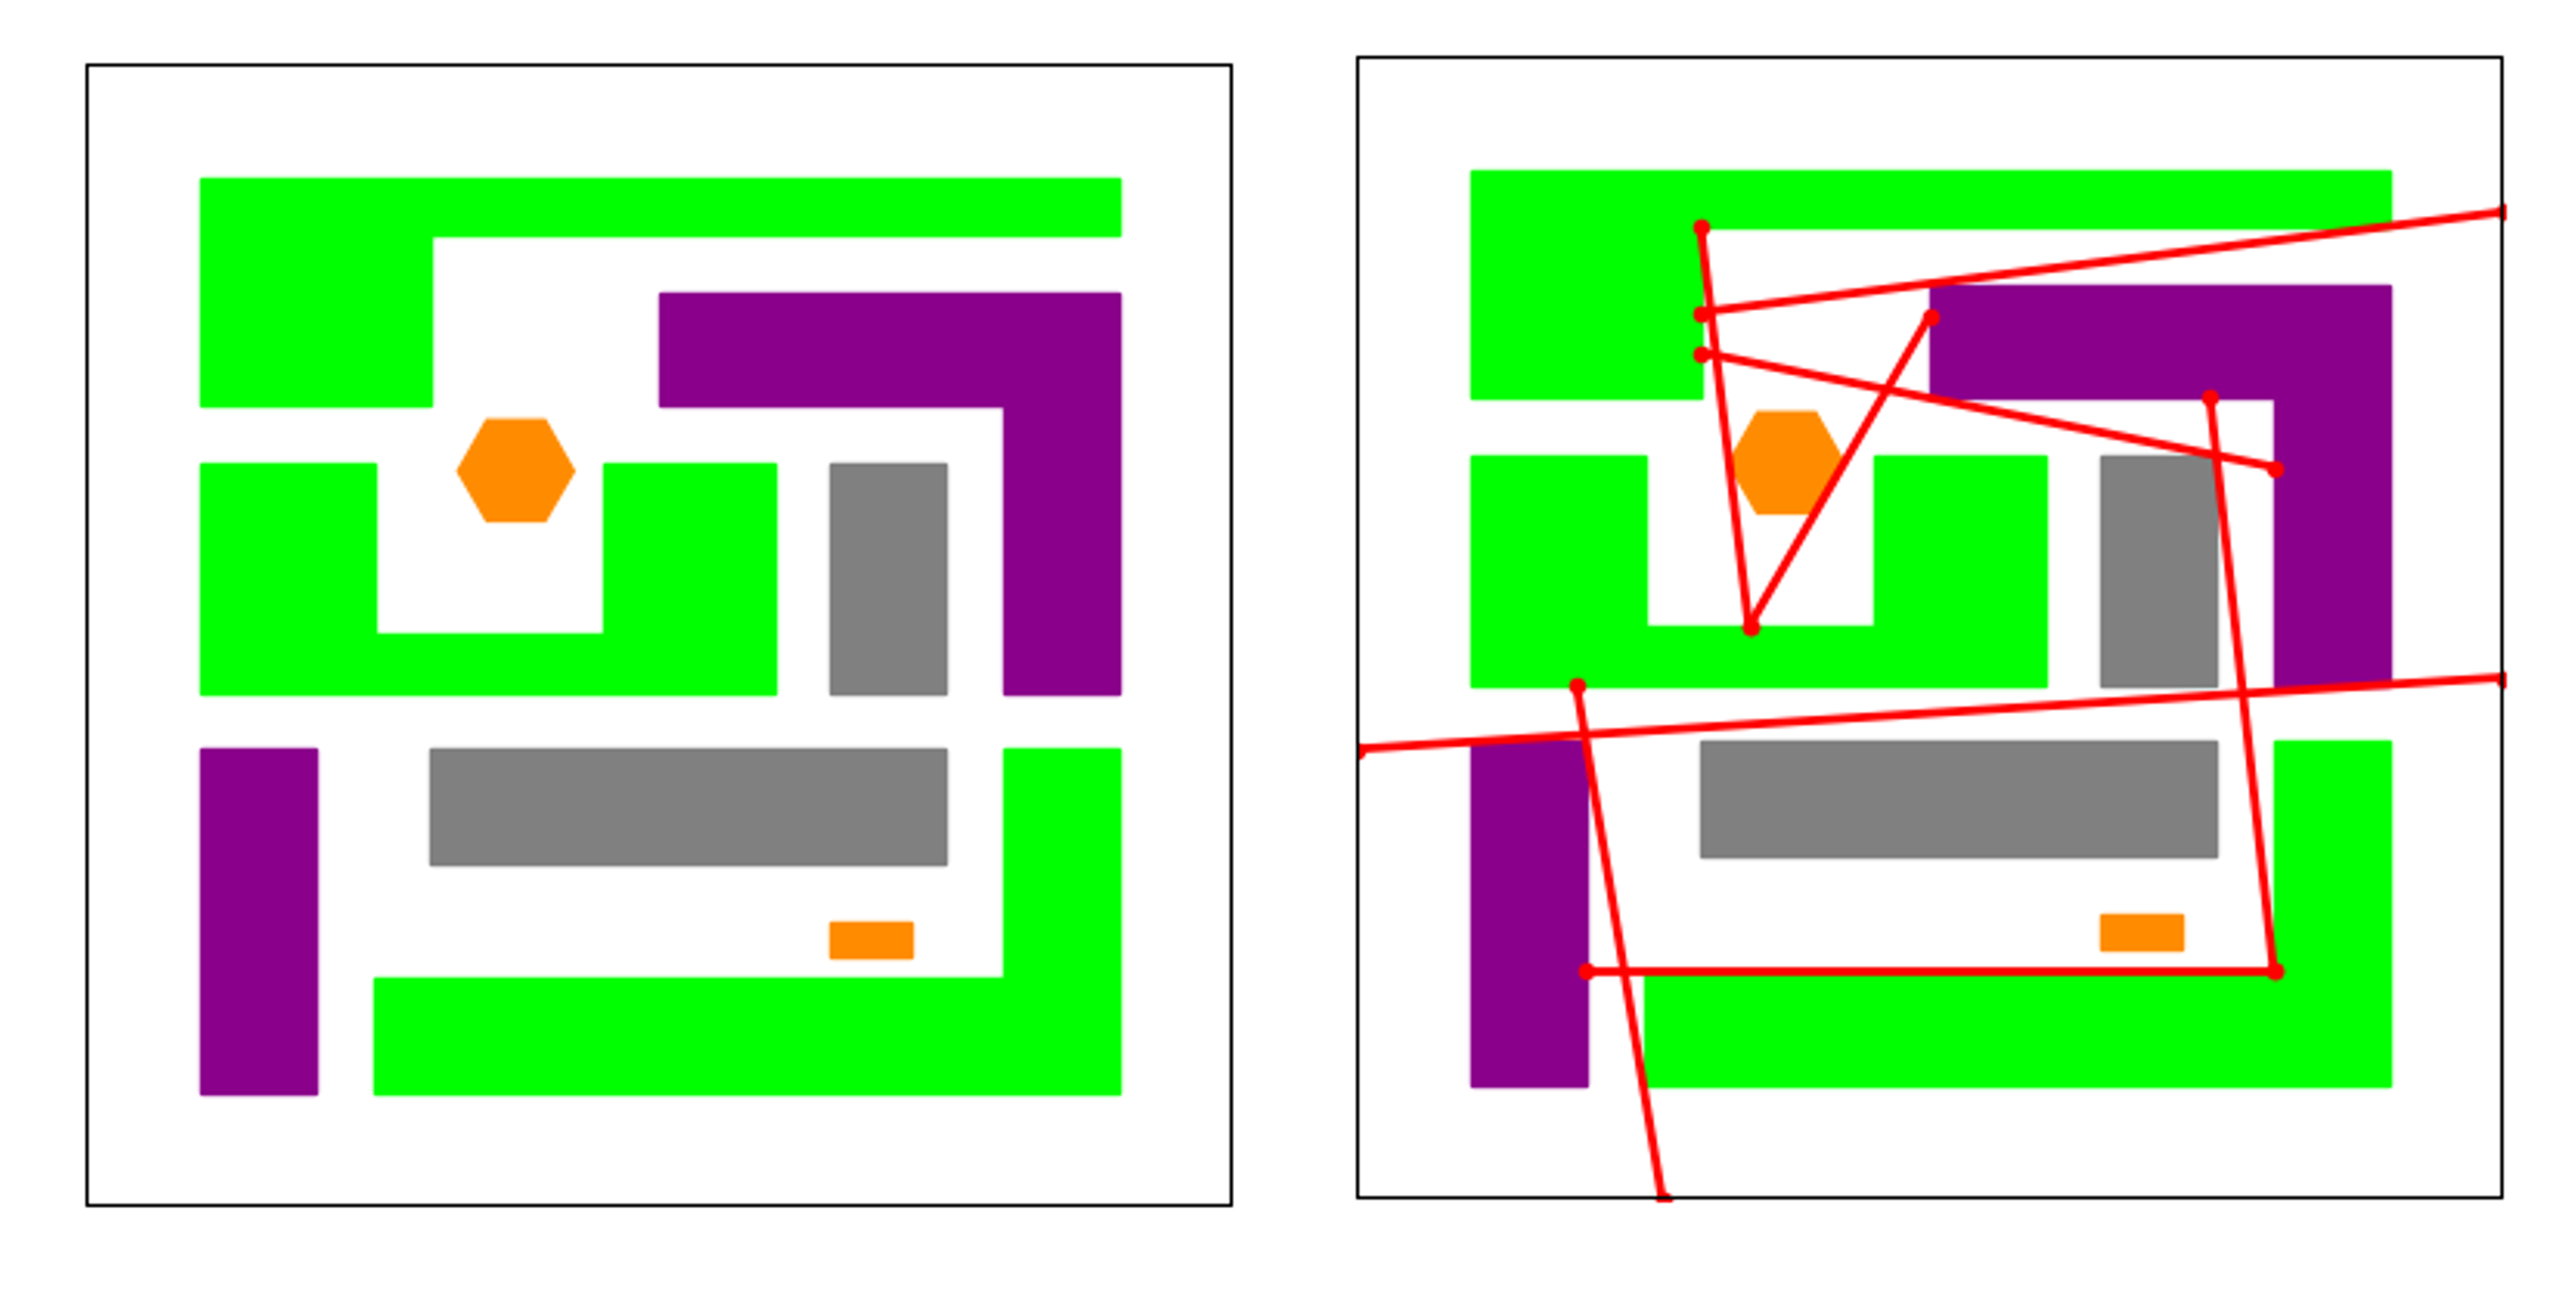
\includegraphics[width=\columnwidth]{chapters/bf/fig/intro_pic.png}
    \caption[Example of barrier forming for separating three sets of complex polygonal shapes]
    {Example of barrier forming for separating three sets of complex polygonal shapes. Different colors represent different sets with the grey ones representing obstacles. The red line segments are the barriers computed by our algorithm.}
    \label{fig:bf-ex}
    \vspace{-0.2in}
\end{figure}
As a summary of this work and its contributions, we study three settings in using line segments to separate sets of disjoint geometric shapes in a 2D workspace: (1) separating point sets, (2) separating point sets among polygonal obstacles, and (3) separating polygonal sets among polygonal obstacles. 
%
Whereas all three settings are NP-hard to optimally solve, we derive an effective method for computing optimal solutions for the first two settings, capable of handling tens of objects (points and/or polygons) partitioned into multiple sets. 
%
The  method first systematically computes candidate barrier set containing a minimum separating barrier, and then builds a novel integer programming model for finding the minimum barrier. 
%
Following a similar approach, we also develop a method that computes solutions for the third set that is proven to be at least $2$-optimal. 
%
We provide a theoretical analysis that sheds some light on why the setting involving polygonal sets is more difficult to solve.
%
Extensive simulation study corroborates the effectiveness of our algorithms. 

%Our contribution to barrier forming is, in summary, formulating the problem of minimizing
%the line segment barriers used with respect to different kinds of object sets (point object and polygonal object). 
%For barrier forming among sets of point objects, we provide effective integer programming based method to obtain the optimal solution.
%For the general polygonal objects, our method can provide a guaranteed 2-OPT solution.
%We also perform evaluations on four different settings to show
%the effectiveness of the proposed method.


\noindent\textbf{Related Work}.
Our investigation of barrier forming has its origins in several research areas.
In the study of pursuit evasion or more generally differential games \cite{ho1965differential,isaacs1999differential,hajek2008pursuit,tovar2009sensor,simov2000pursuit,guibas1997visibility,kameda2006online,kirousis1986searching, sachs2004visibility,lau2005optimal, yu2011shadow, olsen2022robust}, 
% flash light searcher, 1-2 inf searcher
such scenarios often happen where several agents are tasked to search an environment for hidden rogue agents or to protect critical regions from outsider invaders, which amount to creating and maintaining static or dynamic barriers of some form.  
%
Among the approaches taken in finding solutions for these problems, some resort to discretizing the environment into graph representations and conducting search over them \cite{kirousis1986searching, sachs2004visibility}, while others adopt probabilistic reasoning \cite{lau2005optimal, yu2011shadow}. 
%
In particular, Tovar et al. \cite{tovar2009sensor} studied a problem that examines how to untangle sensor beam crossings to reason about the state of a robot, and use the insight to build algorithms for driving a robot to a desired state. In a sense, their study can be viewed as studying a problem that is a dual of the problem that we study here. 

%\textcolor{red}{JJ's edit location}

The barrier forming problem can also be seen as a type of sensor coverage problem. 
%
A series of studies on perimeter defense/guarding problems aim at covering the boundaries of some regions to protect them from the outside \cite{shishika2020cooperative, macharet2020adaptive, fenghangaoyu2019efficient, fengyu2020optimally}, which share similar motivations. 
The barrier forming problem has more flexible solutions by not fixing the specific boundaries to secure the critical regions,
which can be more general and closer to reality in certain cases.
The concept of barrier coverage originates from \cite{gage1992command}, together with the blanket and sweep coverage. 
In \cite{kumar2005barrier}, $k$-barrier was studied. 
In \cite{kloder2007barrier}, the authors solved the min-distance barrier coverage problem optimally under non-trivial environment to minimize the total length of the barriers between two groups of polygonal objects. 
To tackle the proposed problem, a novel and efficient network-flow based method is applied. 
Multiple groups of objects are tackled in \cite{abrahamsen2020geometric}.
The following work \cite{kloder2008thesis} includes a similar problem formation to the problem studied in this chapter, where the objective is minimizing the number of fixed-length line segments used. 
%
However, the proposed method in \cite{kloder2008thesis} uses Tarski sentence \cite{tarski1949decision} which, to our knowledge, does not have a very effective computational tool to deal with.

This work is closely related to several problems in computational geometry, especially point set shattering which seeks a complete separation among a single set of points \cite{freimer1991complexity, har2020separating}. 
Bichromatic point sets or polyhedral separation problem uses wedges, axis-aligned lines, chords, parallel lines, or circles to separate two sets of points or polyhedra \cite{devillers2001separating,armaselu2017geometric,boissonnat2001circular, demaine2005separating}. 
Work on these problems often introduces specific constraints such as working with convex objects or simple polygons without holes, adopting non-crossing or parallel lines as the separator, and so on. 

\noindent \textbf{Chapter Structure}.
The rest of the chapter starts with formulating the barrier formation problem and 
introducing the three variants studied in ~\ref{sec:bf-preliminary}. 
Then, we describe the structure analysis of the problem in ~\ref{sec:bf-structure}, which will base the algorithm
proposed in ~\ref{sec:bf-algorithm}. Lastly, in ~\ref{sec:bf-evaluation} we evaluate the algorithm on four different scenarios. %\r{associate each with a specific section.}

%  methods take
% The problem of constructing a set of barriers appears in various robotics applications 


% Barrier forming is studied in various domains.
% In the pursuit evasion game, barriers were constructed to perform 
% area scan, moving target persuasion \cite{yu2011shadow, tovar2009sensor} etc.
% In computational geometry,
% barrier forming has relevance to several problem: 
% Regarding separating polygons, 
% the study of barrier coverage problem introduces a network flow-based algorithm 
% for computing the minimum total distance separation for two sets of polygons 
% with the existence of obstacles\cite{kloder2007barrier, kloder2008thesis}.
% In \cite{kloder2008thesis}, the author explored barrier forming with minimum number of 
% fixed-length line segments, while it is still important to find high performance
% solution for such problem.\label{sec:bf-intro}

\section{Preliminaries}\label{sec:bf-preliminary}
\subsection{Barrier Forming with Minimum Number of Line Segments}

\begin{figure}[ht]
    \centering
    \vspace{.05in}
    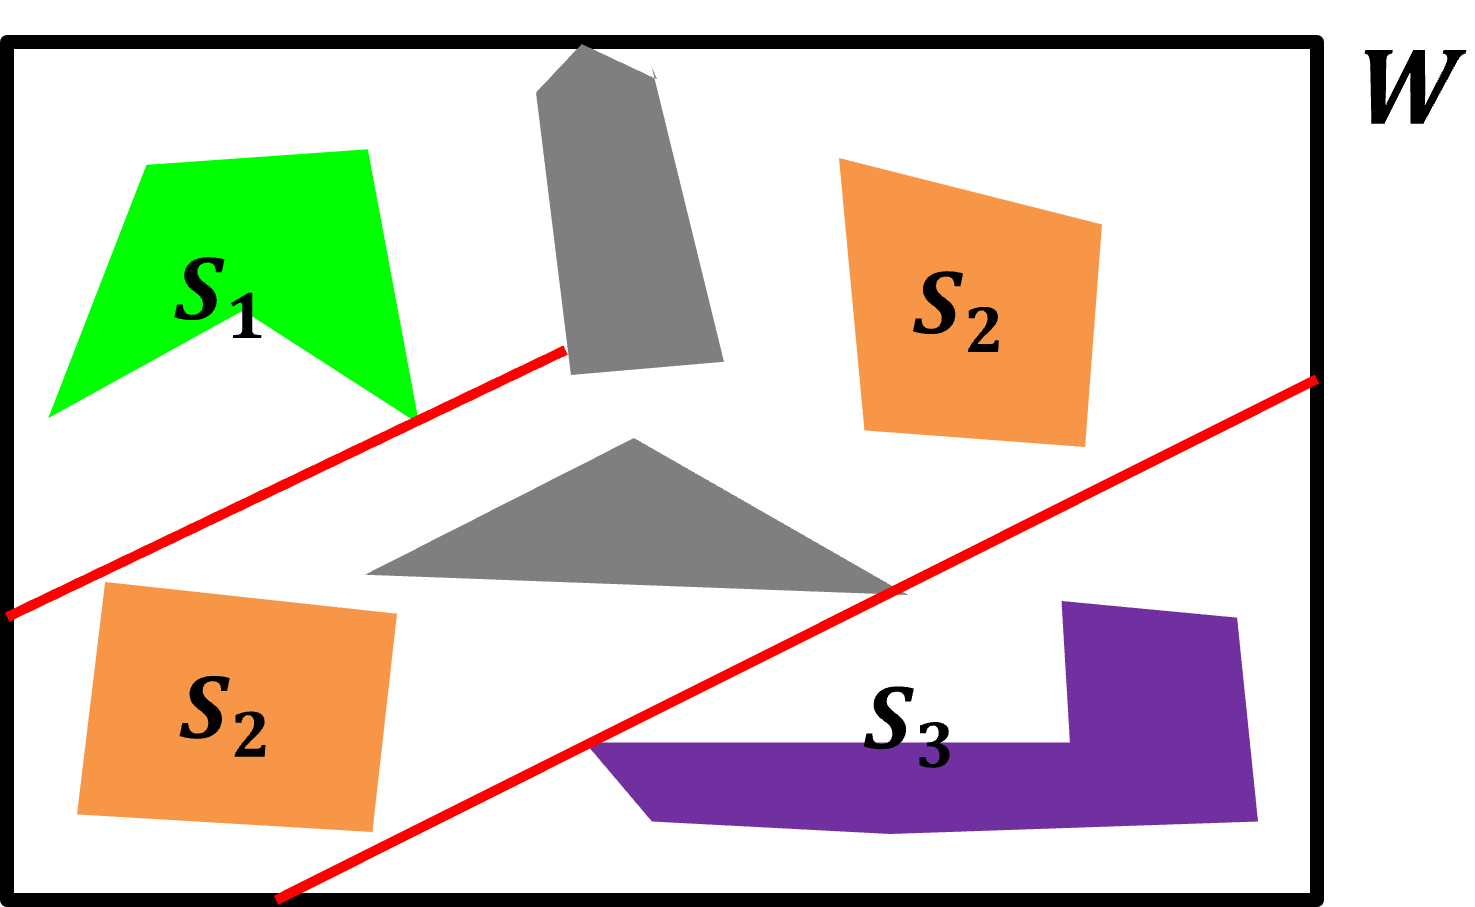
\includegraphics[width = .35\textwidth]{chapters/bf/fig/formulation_pic.png}
    \vspace{.05in}
    \caption[Illustration of a barrier forming problem for the three sets of polygonal objects]
    {Illustration of a barrier forming problem for the three sets of (colored) polygonal objects $S_{1\sim3}$ among (gray) obstacles. 
    For the setting, $2$ straight lines are sufficient to cut off path connections between any pair of polygon regions from two different sets. 
    In this work, our general goal is to build such barriers with the least number of line segments.}
    \label{fig:bf-illustration}
    % \vspace{-0.2in}
\end{figure}

Let $\mathcal{W}$ be a simply connected polygonal workspace in $\mathbb R^2$. Consider $k$ sets of objects $S_1, \dots, S_k$ in $\mathcal W$, as well as a set of polygonal obstacles $\mathcal O$. 
We seek to use a set of straight line segments $L$ to separate $S_1, \dots, S_k$ from each other, such that for any two objects $o_1 \in S_i$ and $o_2 \in S_j, i \ne j$, any path between $o_1$ and $o_2$ in the free space of $\mathcal W$ must be ``cut off'' by one or more line segments from $L$. 
The line segments do not have length limit and can cross each other, but they cannot cross objects or obstacles in the workspace. We want to find the minimum number of line segments to complete the separation task. 

Under the general formulation of Barrier Forming, we examine three different variants with increasing difficulty:
\begin{enumerate} 
\item \emph{Barriers for point sets}, in which  $S_1, \dots, S_k$ as well as $O$ are sets of points. 
\item \emph{Barriers for point sets among polygonal obstacles}, in which  $S_1, \dots, S_k$ are sets of points but $O$ is a set of polygonal objects. 
\item \emph{Barriers for polygonal objects}, in which $S_1, \dots, S_k$ as well as $O$ contain polygonal objects. 
\end{enumerate}
%The first problem considers points sets for separation, that in this case, $S_1, %\dots, S_k$ are point sets, and there are no obstacles in the workspace. This is the %same as the point set separation problem in the plane. 
%The second still takes $S_1, \dots, S_k$ as point set, but introduces polygonal obstacle sets $\mathcal O$ in the workspace. 
%The last one further considers $S_1, \dots, S_k$ as polygonal object sets.

\subsection{Computational Intractability}
Because the separation of even two sets of points in the plane, 
a special case of the first variant of our barrier forming problem, 
is computationally intractable \cite{demaine2005separating}, 
our first formulation is also NP-hard. 
From here, we can reduce from the first variant to other variants involving polygonal shapes by converting each point object to a sufficiently small polygon. Therefore, all three versions of the barrier forming problems studied in this paper are NP-hard. We omit the straightforward details. 

\section{Structural Analysis}\label{sec:bf-structure}

Given that barrier forming problems studied in this work are NP-hard, a natural algorithmic choice for addressing the challenge is through exploring  mathematical programming.
%
To that end, a model must be built that selects from candidate barriers, which in turn requires the construction of a representative set of barrier candidates, a rather non-trivial task. 
%
The set of candidate barriers should satisfy two conflicting constraints: (1) it should contain a minimum set line segments that achieves the desired separation and (2) its size should not be too big that it will cripple the barrier selection process. 
%
Through careful structural analysis, we notice that the barriers to be considered can be limited to \emph{tangent} or \emph{bitangent} line segments. A tangent line segment, with respect to an object or an obstacle, is a line that passes through a vertex or an edge of the object/obstacle but does not intersect its interior. A bitangent is a line segment that is tangent to two objects and/or obstacles. 
%
This allows us to significantly reduce the number of candidates to be examined at the later selection stage.

\begin{theorem}\label{theorem:bf-sin_tan}
For any $k$ sets of polygonal or point objects $S_1, \dots, S_k$ in the workspace $\mathcal W$, the set of line segments that are tangential to the objects and obstacles contains a set of minimum cardinality that separates $S_1, \dots, S_k$. 
\end{theorem}


\begin{proof}

% We prove that there exists a set of lines with minimum cardinality that separates $S_1, \dots, S_k$, and consists of only lines tangent to object vertices. 
Consider a set of line segments $L^*$ with minimum cardinality that separates $S_1,\dots, S_k$. 
Without loss of generality, we assume all line segments in $L^*$ do not end in the free space, i.e., each line segment in $L^*$ ends
at either object boundaries or workspace boundaries.
If some line segment in a minimum barrier is not tangent to any object vertex, denoted it as $\ell=OA$ (shown in ~\ref{fig:bf-proof}), 
we show that it can be replaced by a line segment that is tangent to some object vertex. 
%
Fix one end of $\ell$, $O$ in this case, and rotate $\ell$ around $O$ in both clockwise and counterclockwise directions until it hits some object vertex and becomes tangential to the object.
%
Denote the two line segments resulting from clockwise rotation and counterclockwise rotation as $\ell_1'=OB$ and $\ell'_2=OC$, respectively. 

We show $\ell$ can be replaced with $\ell_1'$ or $\ell_2'$. 
If this is not the case,
since replacing $\ell$ with $\ell_1'$ cannot make the separation work, there must be some point $P_1$ between $AB$ that is path connected to some point in the other class without crossing any line segments in $L^*$ when $\ell$ is replaced with $\ell'_1$. Denote the point as $D_1$ and the path as $path_1$. 
The same analysis goes for $\ell'_2$, that if $\ell$ cannot be replaced by $\ell_2$ then there is some point $P_2$ in $AC$ and path $path_2$ that connects $P_2$ to some other point $D_2$ in a different class and crosses segment $\ell$ but not $\ell_2'$. 
Since there are no objects or obstacles inside triangle $OCB$, we can assume the parts of $path_1$ and $path_2$ inside triangle $OCB$ are straight lines.
So, $path_1$ and $path_2$ must cross each other at some point. 
Denote the cross point as $Q\in path_1 \cap path_2$. 
Then, $path_1 = path_{11} (from\ P_1\ to\ Q) + path_{12} (from\ Q\ to\ D_1)$ and $path_2 = path_{12} (from\ P_2\ to\ Q) + path_{22} (from\ Q\ to\ D_2)$. 
Path $p_{11} + p_{22}$ connects $P_1$ to $D_2$, and $p_{21} + p_{12}$ connects $P_2$ to $D_1$, one of which must not cross $\ell$. 
This leads to a contradiction to the fact that the original line set $L^*$ separates the $k$ classes of objects.

Therefore, each non-tangent line segment in $L^*$ can be replaced with a tangent line segment. 
It will eventually result in a set of tangent barriers with minimum cardinality that separates $S_1,\dots,S_k$.
\begin{figure}[ht]
    \vspace{-2mm}
    \centering
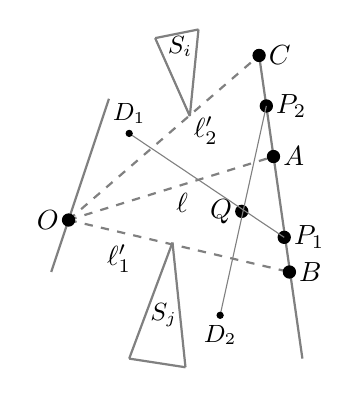
\begin{tikzpicture}[scale = 1.1]
\draw[gray, thick] (0.1, 0) -- (0.7666, 2);
\draw[gray, thick] (3, -1) -- (2.5, 2.5);


\draw[gray, thick] (1, -1) -- (1.5, 0.34);
\draw[gray, thick] (1.65, -1.1) -- (1.5, 0.34);
\draw[gray, thick] (1.65, -1.1) -- (1, -1);

\draw[gray, thick] (1.3, 2.7) -- (1.7, 1.8);
\draw[gray, thick] (1.8, 2.8) -- (1.7, 1.8);
\draw[gray, thick] (1.8, 2.8) -- (1.3, 2.7);

\draw[gray, thick, dashed] (0.3, 0.6) -- (2.66666, 1.333);

\draw[gray, thick, dashed] (0.3, 0.6) -- (2.5, 2.5);
\draw[gray, thick, dashed] (0.3, 0.6) -- (2.85, 0);

\node[text width=1cm] at (2, 0.8) {$\ell$};
\node[text width=1cm] at (2.2, 1.63) {$\ell_2'$};
\node[text width=1cm] at (1.2, 0.15) {$\ell_1'$};

\filldraw[black] (0.3, 0.6) circle (2pt) node[anchor=east] {$O$};
\filldraw[black] (2.666, 1.333) circle (2pt) node[anchor=west] {$A$};
\filldraw[black] (2.5, 2.5) circle (2pt) node[anchor=west] {$C$};
\filldraw[black] (2.85, 0) circle (2pt) node[anchor=west] {$B$};

\filldraw[black] (2.79, 0.4) circle (2pt) node[anchor=west] {$P_1$};
\filldraw[black] (2.5833, 1.917) circle (2pt) node[anchor=west] {$P_2$};

\filldraw[black] (2.3, 0.7) circle (2pt) node[anchor=east] {$Q$};

\draw[gray] (2.79, 0.4) -- (1.0, 1.6);
\draw[gray] (2.5833, 1.917) -- (2.05, -0.5);
\filldraw[black] (1.0, 1.6) circle (1pt) node[anchor=south] {\small{$D_1$}};
\filldraw[black] (2.05, -0.5) circle (1pt) node[anchor=north] {\small $D_2$};


\node[text width=1cm] at (1.9, 2.6) {\small $S_i$};
\node[text width=1cm] at (1.7, -0.5) {\small $S_j$};

\end{tikzpicture}
    \caption{Rotating non-tangent barrier line segment $\ell$ in clockwise and counterclockwise directions around its endpoint $O$ until it becomes tangential to some objects.}
    \label{fig:bf-proof}
    \vspace{-2mm}
\end{figure}
% Then, we show that there exists a set of lines with minimum cardinality that separates $S1$ and $S2$. Similarly, when a line is only tangent to one vertex
\end{proof}

Although we can limit the candidate barriers to line segments tangent to object vertices, there can
still be infinite number of candidates. 
One may consider using line segments that are bitangent to
object vertices, i.e. line segments crossing two object or obstacle vertices. 
If there are $n$ object/obstacle vertices, there can be at most $n^2$, i.e., a quadratic number of bitangents. 
Unfortunately, bitangent lines are insufficient to act as candidate barriers by themselves for polygonal objects. 
A counterexample in ~\ref{fig:bf-counter} shows that there is an instance where an optimal solution must contain line segments that are not bitangents. 
%
In this counterexample, we need separate the orange objects from the lime object. A minimum of three line segments are used, 
and it is not possible that all of them are bitangent, i.e.

\begin{proposition}
Bitangent line segments do not always contain optimal solution for the barrier forming problem for polygonal objects.
\end{proposition}

\begin{figure}[ht]
    \centering
    \vspace{-.2in}
    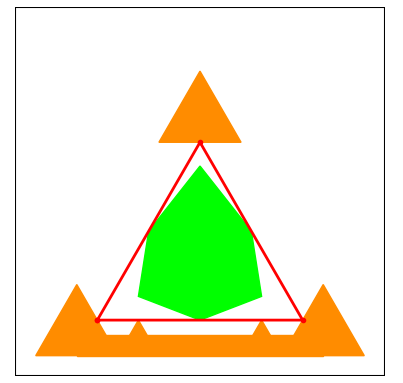
\includegraphics[width = .25\textwidth]{chapters/bf/fig/counter_example.png}
    \vspace{0.0in}
    \caption{Counterexample that shows using only bitangent line segments cannot create the optimal solution}
    \label{fig:bf-counter}
\end{figure}

Despite the caveat, for the first two formulations that deal with barrier forming for point sets, even with polygonal obstacles, bitangent line segments
always contain an optimal solution. More precisely, 
\begin{theorem}
For any $k$ sets of point objects $S_1, \dots, S_k$ in a workspace $\mathcal W$, there exists
a set of line segments with minimum cardinality that separates $S_1, \dots, S_k$, 
and only consists of bitangent line segments.
\end{theorem}

\begin{proof}
From Theorem~\ref{theorem:bf-sin_tan}, we can see using single tangent line segments is always enough
for an optimal solution. 
Now we turn an optimal solution, $L^*$, with only tangent line segments, into
a solution with only bitangent line segments while still maintaining the same number of barriers. 

For a tangent line segment $\ell=AB\in L^*$ with tangent point $O$ (shown in ~\ref{fig:bf-proof_bi}), and if $O$ is a point object, assume it is beneath $\ell$,
rotate $\ell$ clockwise around $O$ until it hits a point object or an obstacle vertex.
Denote the resulting line segment as $\ell'$, and replace $\ell$ with $\ell'$.
Since the objects are point objects, so $BB'$ and $AA'$ must belong to obstacles or workspace boundary, 
and thus there is no object point inside $OAA'$ or $OBB'$. 
Therefore, the replacement won't result in
any path connecting objects in different classes.
If this is not the case, then there will be some path connecting two object points in different classes that crosses $\ell$ but does not cross $\ell'$ or other barriers. 
Since the triangle areas $OAA'$ and $OBB'$ are empty, that path must enter region $OAA'$ or $OBB'$ and leave them from $\ell$. Then, that part of the path could be replaced with a straight line segment parallel to $\ell$ which prevents it from crossing $\ell$. This contradicts the assumption that $L^*$ prevents all connections between objects in different classes. % of objects.

Continuing the replacement until all line segments are bitangent will result in an optimal solution with only bitangent line segments.

\begin{figure}[ht]
    \centering
    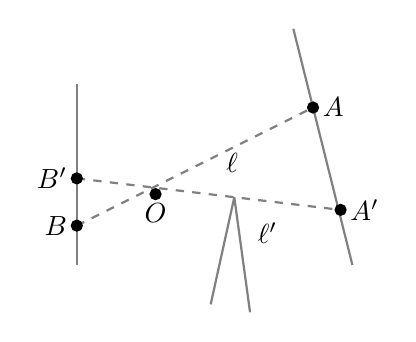
\begin{tikzpicture}
    % \draw[gray, thick] (0, 0) -- (1, 2);
    \draw[gray, thick] (2.5, -1) -- (1.75, 2);
    \draw[gray, thick] (-1, -1) -- (-1, 1.3);

    \draw[gray, thick] (0.7, -1.5) -- (1, -0.14);
    \draw[gray, thick] (1.2, -1.6) -- (1, -0.14);

    % \draw[gray, thick] (3, -1) -- (2.5, 2.5);

    % \draw[gray, thick] (1, -1) -- (1.5, 0.34);
    % \draw[gray, thick] (1.65, -1.1) -- (1.5, 0.34);
    % 
    % \draw[gray, thick, dashed] (0.3, 0.6) -- (2.66666, 1.333);
    \draw[gray, thick, dashed] (-1., -0.5) -- (2., 1.);

    \draw[gray, thick, dashed] (-1., 0.1) -- (2.35, -0.3);

    % \draw[gray, thick, dashed] (0.3, 0.6) -- (2.5, 2.5);
    % \draw[gray, thick, dashed] (0.3, 0.6) -- (2.85, 0);

    \node[text width=1cm] at (1.4, 0.3) 
                            {$\ell$};
    % \node[text] at (1.8, 1.63) 
                            % {$\ell_2'$};
    \node[text width=1cm] at (1.8, -0.6) 
                            {$\ell'$};

    \filldraw[black] (0.0, -0.1) circle (2pt) node[anchor=north] {$O$};
    \filldraw[black] (2, 1.) circle (2pt) node[anchor=west] {$A$};
    % \filldraw[black] (2.5, 2.5) circle (2pt) node[anchor=west] {$C$};
    \filldraw[black] (-1, -0.5) circle (2pt) node[anchor=east] {$B$};

    \filldraw[black] (2.35, -0.3) circle (2pt) node[anchor=west] {$A'$};
    \filldraw[black] (-1, 0.1) circle (2pt) node[anchor=east] {$B'$};

    % \filldraw[black] (2.7583, 0.6666) circle (2pt) node[anchor=west] {$P_1$};
    % \filldraw[black] (2.5833, 1.917) circle (2pt) node[anchor=west] {$P_2$};

    \end{tikzpicture}
    \caption{Rotating a single tangent barrier line segment $\ell$ around its tangent point $O$ clockwise until it becomes bitangent.}
    \label{fig:bf-proof_bi}
\end{figure}
\end{proof}

For separating polygonal objects, although using bitangent line segments cannot guarantee an optimal solution that uses minimum number of line segments, they can still ensure that solutions limited to bitangents are at least $2$-optimal.
\begin{proposition}
For any $k$ sets of polygonal objects $S_1, \dots, S_k$ in the workspace $\mathcal W$, there exists a set of line segments with cardinality at most twice the minimum cardinality, that separates $S_1, \dots, S_k$, and only consists of line segments that are bitangent to object or obstacle vertices. 
\end{proposition}
\begin{proof}


\begin{figure}[ht]
    \centering
    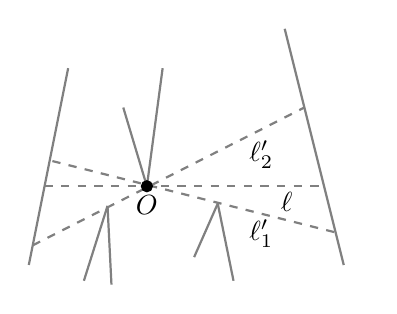
\begin{tikzpicture}

    \draw[gray, thick] (2.5, -1) -- (1.75, 2);
    \draw[gray, thick] (-1.5, -1) -- (-1, 1.5);
    \draw[gray, thick] (0, 0) -- (-0.3, 1);
    \draw[gray, thick] (0, 0) -- (.2, 1.5);

    \draw[gray, thick] (-0.8, -1.2) -- (-0.5, -0.25);
    \draw[gray, thick] (-0.45, -1.25) -- (-0.5, -0.25);

    \draw[gray, thick] (0.6, -0.9) -- (0.9, -0.22);
    \draw[gray, thick] (1.1, -1.2) -- (0.9, -0.22);


    \draw[gray, thick, dashed] (-1.45, -0.75) -- (2., 1.);
    \draw[gray, thick, dashed] (-1.3, -0.0) -- (2.2, 0);

    \draw[gray, thick, dashed] (-1.2, 0.32) -- (2.45, -0.6);



    \node[text width=1cm] at (2.2, -0.2) 
                            {$\ell$};

    \node[text width=1cm] at (1.8, -0.6) 
                            {$\ell'_1$};

    \node[text width=1cm] at (1.8, 0.4) 
                            {$\ell'_2$};

    \filldraw[black] (0.0, -0.0) circle (2pt) node[anchor=north] {$O$};


    \end{tikzpicture}
    \caption{Rotating tangent barrier line segment $\ell$ both clockwise and counterclockwise around its tangent point $O$ until it becomes bitangent.}
    \label{fig:bf-proof_bi_2opt}
\end{figure}

Starting from an optimal solution $L^*$ with only tangent line segments,
we will replace each tangent line segment with two bitangent line segments.

Rotate each non-bitangent line segment $\ell\in L^*$ around its tangent point $O$ in clockwise or 
counterclockwise directions until the line segment become bitangent, 
as illustrated in ~\ref{fig:bf-proof_bi_2opt}. 
Since any path connecting two objects in different classes and is cut by barrier $\ell$ will still be cut by $\ell'_1$ and $\ell'_2$.
The replacement can still guarantee the separation among the object groups.
After replacing all barriers, we can obtain a 2-OPT solution with the number of line segments twice the minimum.
\end{proof}


\section{Fast Computation of High-Quality Solutions}\label{sec:bf-algorithm}
In this section, we will apply the structural results of the barrier forming problem and provide effective method to tackle it.
First, we start with a general method for obtaining the optimal solution among a set of candidate barriers.
Then, based on different ways to generate the candidate barriers, two approaches are given while one is based on 
using bitangent line segments and the other is based on sampling.

\subsection{Optimal Solution for Given Line Separator Candidates}
\label{sec:bf-algo:ilp}
In the barrier forming problem, if the candidate barriers are available as a finite set, we can tackle the problem with integer programming (IP). 
To solve it, we first perform a decomposition of the workspace using the candidate barriers, which partitions the workspace into cells whose edges are part of some candidate barriers. 
Denote  $N$ as the number of candidate barrier line segments, and $M$ as the number of 
cells dissected using the candidate barriers. ~\ref{fig:bf-ilp_example} shows an example of dissecting the workspace into six cells with three candidate barriers.
Then, we can start to construct an IP model to solve the problem of minimizing the number of selected barriers. 
First, we use $\lceil\log k\rceil$ binary variables for each cell, 
resulting in $M\cdot\lceil \log k \rceil$ such variables $c_{11}, \dots, c_{M\lceil\log k\rceil}$. 
The value of $\overline{c_{i1}c_{i2}\dots c_{i\lceil \log k\rceil}}$ will represent the class of cell $i$. 
Thus, if there is an object in cell $i$, $\overline{c_{i1}c_{i2}\dots c_{i\lceil \log k\rceil}}$ should have a fixed value according to the class of the object.
A binary variable for each candidate line segment is used to indicate whether that line candidate is selected,
resulting in $N$ such variables: $\ell_1, \dots, \ell_N$. 

\begin{figure}
    \centering
    \begin{overpic}[width=0.3\textwidth]{chapters/bf/fig/ilp_example.png}
    \put(0, 60) {$\ell_1$}
    \put(40, 95) {$\ell_2$}
    \put(55, 95) {$\ell_3$}
    
    \put(15, 80) {$c_1$}
    \put(50, 75) {$c_2$}
    \put(80, 80) {$c_3$}
    \put(15, 30) {$c_4$}
    \put(50, 15) {$c_5$}
    \put(80, 30) {$c_6$}
    \end{overpic}
    % \includegraphics
    \caption{In this example, we aim to separate two groups of objects with the given candidate barriers. The workspace is decomposed into 6 cells by the 3 candidate barriers. As an example of constraint setup, the pair of adjacent cells $c_1$ and $c_4$ create a constraint of
    $\ell_1\geq c_1 \oplus c_4$, which is equivalent to $\ell_1\geq c_1 - c_4 \wedge \ell_1\geq c_4 -c_1$. (Since there is only $k=2$ classes of objects and $\log k =1$ here, the second index of $c_{i*}$ is eliminated.)} 
    \label{fig:bf-ilp_example}
\end{figure}

Between each pair of adjacent cells $i$ and $ j$ (let the candidate line segment between them correspond to $\ell_\sigma$), we have ($\oplus$ denotes ``exclusive or'')
\begin{equation}
\begin{split}
    &\ell_\sigma \geq c_{i\tau} \oplus c_{j\tau}  \Leftrightarrow \ell_\sigma \geq c_{i\tau} - c_{j\tau} \wedge \ell_\sigma\geq c_{j\tau} - c_{i\tau}, \\
    &\text{  for each adjacent cell $i$, $j$, and $1\leq \tau \leq \lceil \log k \rceil$},
\end{split}
\end{equation}
which means if two adjacent cells belong to different classes, then the line segment candidate between them must be selected. 
An example of the constraint setup is illustrated in ~\ref{fig:bf-ilp_example}.
Naturally, we have fixed $c_{i1},\dots,c_{i\lceil \log k\rceil}$ if ceil $i$ contains an object to be separated, 
and the value of $\overline{c_{i1}c_{i2}\dots c_{i\lceil \log k\rceil}}$ is set to be the same as its class index: $0\sim k-1$.
The objective is set to minimize the total number of line candidates selected, i.e., $\min \sum_{i=1}^{M} l_i$.

\subsection{Near-optimal Solution Using Bitangent Lines}
As the results in Section~\ref{sec:bf-structure} show, using bitangent line segments 
can always provide optimal solution for the problem of barrier forming for point objects, 
and at least 2-OPT
solution for separating polygonal objects. 
Since the number of bitangent line segments is at 
most quadratic to the number of object or obstacle vertices, 
we can enumerate them, and apply IP method in Section~\ref{sec:bf-algo:ilp} to find a solution. 
~\ref{fig:bf-barrier_candidates} illustrates the candidate barriers constructed for point objects and polygonal objects.
It is worth noting that for enumerating bitangent barriers for point objects, the side of the point to the barrier also matters. 
For example, a pair of point objects will create $4$ bitangent barrier candidates as there are 4 different possible cases depending on the how the corresponding objects are placed with respect to the line. 

\begin{figure}[ht]
    \centering
    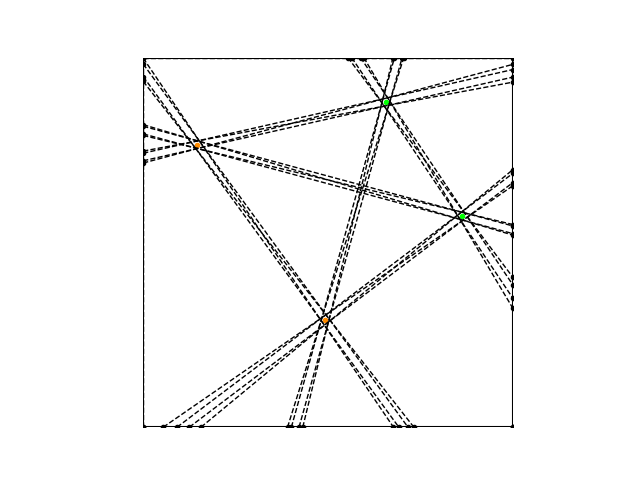
\includegraphics[trim=80 20 80 20,clip, width = .24\textwidth]{chapters/bf/fig/candidate_1.png}
    \hspace{-.1in}
    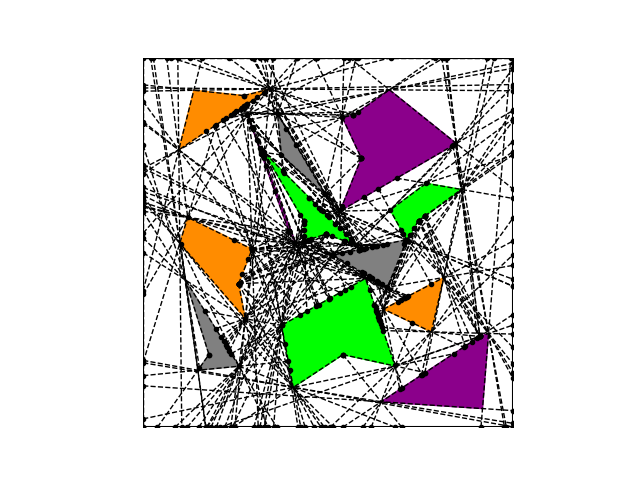
\includegraphics[trim=80 20 80 20,clip, width = .24\textwidth]{chapters/bf/fig/candidate_2.png}
    \caption{Illustration of bitangent barrier candidates. The left picture shows the bitangent
    candidates for $2$ point sets, each with $2$ points. In this case, a pair of points will create $4$ candidates. 
    We note that we made the points non-zero-dimensional for visibility purposes. 
    The right picture shows the bitangent candidates for $12$ polygonal objects in four sets.}
    \label{fig:bf-barrier_candidates}
\end{figure}

\subsection{Sampling-based Resolution Complete Algorithm}
Although using bitangent line segments works well in most of the cases, it unfortunately cannot provide an optimal guarantee for the barriers formed when dealing with polygonal objects.
However, theorem~\ref{theorem:bf-sin_tan} provides a good starting point for sampling line segments: we may limit candidate barrier sets to single tangents, 
i.e., we sample line segments passing through each object vertex in a radial manner. 
Hence, if we gradually increase the sampling resolution around each object and obstacle vertex and use the sampled line segments as candidate barriers, 
we can guarantee the asymptotic optimality of the resulting solution.

% In this section, we first describe a polynomial time approximation algorithm for a restricted version of Problem~\ref{p:2}. Then, we describe a general integer linear programming framework for solving Problems~\ref{p:1}-\ref{p:3},
% and local improvement techniques for enhancing solution quality.

% \subsection{Polynomial Time Approximation Algorithm}
% % Briefly mention the hardness results
% % As for 2D OSG, it is similar to the metric k-center problem and therefore
% the approximation algorithms solving k-center problem can be applied to 2D OSG. 

In their general forms, Problems~\ref{p:1}-\ref{p:3} require the computation of 3D visibility, a hard task on its own. Due to this reason, a polynomial time algorithm with guaranteed good approximation ratio for these problems appear difficult to come by. It is an interesting question to ask whether some form of approximation scheme can be derived. Here, we show that for Problem~\ref{p:2}, if one relax the visibility requirement, i.e. letting $vis(\cdot, \cdot)\equiv 1$, then a polynomial time $(2+\varepsilon)$-approximation algorithm can be obtained. 

Taking Problem~\ref{p:2}, we examine a setup assuming that each point $p \in S$ has good visibility, i.e., $p$ is always visible to the nearest sensor. Such scenarios happen when the 3D domain does not have large curvatures that would easily block sensors' view, e.g., covering the earth with GPS satellites or using drones to survey a vineyard. To drive a specific approximation bound, 
we further assume that sensors have spherical range sensing and are in a plane of some fixed 
\begin{wrapfigure}[5]{r}{1.3in}
  \vspace*{0mm}
  \begin{overpic}[width=1.3in,tics=5]{chapters/surf/fig/env.png}
	\end{overpic}
\vspace*{-6.5mm}
\end{wrapfigure}
height $h$ from the ground, which may be relaxed. Denote this surface as $H_C$. 
The figure on the right provides an illustration of the target environment setting. 

The main idea is to first obtain a dense sample of $S$ and then adapt $2$-approximation algorithms for the corresponding 2D setting, which requires some non-trivial reasoning. Two well-known approximation algorithms for $k$-center like problem in 2D are based on \emph{farthest point clustering} \cite{gonzalez1985clustering} and \emph{dominating set} \cite{hochbaum1985best, vazirani2013approximation}. Both of these approaches work for our purpose; we show how to work with the former.

Let a uniformly sampled set of point of $S$ be $S_N = \{o_1, \ldots, o_N\}$. We apply farthest point clustering \cite{gonzalez1985clustering} on $S_N$ as follows. As the name suggest, it picks farthest sensor locations until the number of sensors are exhausted. In the original approach, the points to be clustered are also sensor locations, which is not true here. Instead, we perform clustering in the set $S_N$ and project the selected samples to $H_C$ gradually. The relatively straightforward process is given in Algorithm~\ref{alg:greedy} (($d(\cdot$,$\ \cdot)$ denotes the distance between the inputs, one or both of which may be sets).


\begin{algorithm}
\begin{small}
    \SetKwInOut{Input}{Input}
    \SetKwInOut{Output}{Output}
    \SetKwComment{Comment}{\% }{}
    \caption{Farthest Point Clustering}
		\label{alg:greedy}
    \SetAlgoLined
		\vspace{1mm}
    \Input{$S_N$=\{$o_1, \dots, o_N$\}: $N$ sampled points on the surface $S\subset \partial \mathcal E$; $k$: number of sensors;\\
    $H_C$: a plane with a fixed height}
    \Output{$\mathcal{C}$: sensor location set}
		\vspace{1mm}
        % $\mathcal C$ = $\varnothing$\\
        $\mathcal{C} \leftarrow$  \{$o_1$'s vertical projection onto $H_C$\}\\
        % \While{$|\mathcal{C}|<k$}{
        \For{$i \gets 1$ \KwTo $k$}{
        \For{$o\in S_N$}{
        compute the distance $d(o, \mathcal{C})$ between $o$ and $\mathcal{C}$\\ 
        }
        $o \leftarrow$ point $v\in S_N$ with the largest $d(v,\mathcal{C})$\\
        $\mathcal{C} \leftarrow \mathcal{C}\ \cup \{o$'s projection onto $H_C$\}\\
        % $p^\star \leftarrow$ the projection of $v^\star$ on height $H$\\
        % Add $p^\star$ to $\mathcal{C}$\\
        }
        \Return $\mathcal{C}$
\end{small}
\end{algorithm}

To prove the claimed $(2+\varepsilon)$-approximation bound,  
denote the optimal sensor location set and the sensor location set derived by Algorithm~\ref{alg:greedy} as $\mathcal{C}_{OPT}$ and $\mathcal{C}$, respectively. Since these are centers of spherical sensing ranges, we call them center set for short. Denote the minimum coverage radius in the spherical sensing model as $r_{OPT}$. Let $h$ be the minimum distance between surface $S$ and sensor space $H_C$, i.e. $h:=d(S,H_C)$. $r_{OPT}$ and $r_{\mathcal{C}}$ are defined as follows:
\begin{equation}
    r_{OPT}:=\max_{o\in S_N} d(o, \mathcal{C}_{OPT})
\end{equation}
\begin{equation}
    r_{\mathcal{C}}:=\max_{o\in S_N} d(o, \mathcal{\mathcal{C}})
\end{equation}

\begin{proposition}
\label{prop:algo1t}
The center set obtained by Algorithm~\ref{alg:greedy} achieves coverage radius of at most
%$r_{OPT} + \sqrt{r_{OPT}^2 - h^2}$
$\sqrt{4r_{OPT}^2 - 3h^2}$.
\vspace{-1mm}
\end{proposition}
\begin{proof}

%So we need to prove:
%\begin{equation}
%    r^{C}\leq 2r^{OPT}
%\end{equation}

Denote the center set generated at the 
$i$th round as $\mathcal{C}_{i}$, and $r_i$ as the cluster radius $r_i := \max_{o_\tau}\min_{c_j \in \mathcal{C}_i} d(o_\tau, c_j)$. It is straightforward to observe that $r_k\leq r_{k-1} \leq \dots \leq r_1$.
Consider the relationship between the optimal center set $\mathcal{C}_{OPT}$ and the center set obtained by Algorithm~\ref{alg:greedy}, we have the following 2 cases.

Case 1: For each sphere $\mathcal{B}_{c}$ centered at a point $c\in\mathcal{C}_{OPT}$ with radius of $r_{OPT}$, the projection of $\mathcal{B}_{c}\bigcap S$ onto the sensor space $H_C$
contains exactly one point of $\mathcal{C}_k$. 

% \kg{KG: Since we have a projection step, the OPT sphere needs to cover not only the center, but also the points that project to the center}

In this case, let $v$ be an arbitrary point in $S$. 
Let $c_{\alpha}$ be the nearest center to $v$ in $\mathcal{C}_{OPT}$ 
and $c_{\beta}$ be the point in $\mathcal{C}_k$ whose projection on $S$ is inside $\mathcal{B}_{c_{\alpha}}$. 
Therefore, we have: 
\begin{equation}
    d(v, c_\beta) 
    % \leq d(v,c_{\alpha}) + d(c_{\alpha}, c_\beta) 
    \leq 
    %r_{OPT} + \sqrt{r_{OPT}^2-h^2}
    \sqrt{4r_{OPT}^2 - 3h^2}
\end{equation}

Case 2: There exists a sphere $\mathcal{B}_{c}$ centered at a point $c\in\mathcal{C}_{OPT}$ with radius of $r_{OPT}$, the projection of $\mathcal{B}_{c}\bigcap S$ onto the sensor space $H_C$
contains at least 2 points of $\mathcal{C}_k$. 
In this case, denote the two centers by $c_i$ and $c_j$ $(i<j)$, and their projections on $S$ are in the same sphere $\mathcal{B}_c$. As $c_j$ is added after $c_i$, then,
%Without loss of generality, we can assume that $c_2$ is added in the $i^{th}$ iteration and is no less than $c_1$.% then we have:
\begin{equation}
    \begin{split}
    r_\mathcal{C} = r_k 
    &\leq r_{j}
    \leq d(c_i, c_j\text{'s projection on } S)\\
    &\leq \sqrt{4r_{OPT}^2 - 3h^2}
    % \\
    % &\leq \sqrt{r_{OPT}^2 - h^2} + r_{OPT}\\
    \end{split}
\end{equation}
Summarizing the two cases proves Proposition~\ref{prop:algo1t}.
\vspace{-2mm}
\end{proof}

% \begin{remark}
% With a finer analysis, it can be shown both approximation algorithms are guaranteed to produce at most $\sqrt{4r_{OPT}^2 - 3h^2}$ spherical radius.
% \end{remark}
\vspace{-0.05in}

% \vspace{-2mm}
% \subsection{Integer Programming-Based Algorithmic Framework}
% With Problems~\ref{p:surf-1}-\ref{p:surf-3} being computationally intractable, a natural algorithmic alternative is mathematical programming. In \cite{fengyu2020optimally}, an integer linear programming (ILP) model was shown to be effective for a 2D setting. For our 3D problems, visibility constraints must be effectively handled. We pre-compute pairwise visibility at a given sample granularity. The information is then fed to an ILP model. As the discretization granularity gets smaller, we can then realize \emph{globally optimal} $(1\pm \varepsilon)$-approximations (depending whether it is a maximization or a minimization). 

As a first step to building the ILP model, visibility information must be computed. 
We work with two discretizations, the surface $S$ to be covered and the space where the sensors may be deployed (as discussed in Section~\ref{sec:surf-preliminary}, this is a 3D space though in practice it is frequently a 2D subset). For each pair of samples, we use a collision checker \cite{cgal:aabb-20b} to determine whether the line segments between the two samples intersects $\mathcal E$. During the process, we also compute for each sample $p\in S$ its normal $\hat{n}_p$.

%For the actual computation, we first work only with samples of $S$. For each sample $p \in S$, we then sample the $2$-sphere $\mathbb S^2$ around $p$ to get a unit vector $\vec{v}$. For each $(p, \vec{v})$, we compute the point $p' \in \mathcal E$ that blocks the ray starting at $p$ in the direction of $\vec{v}$. This information is then used to compute pairwise visibility information between the surface samples and sensor location samples. Such an approach decouples the visibility computation between the two sample sets. 

%
With the visibility pre-computation performed, we are ready to construct the ILP models. For all three problems, recall that we have $S_N = \{o_1, \ldots, o_N\}$ for discretizing the surface $S$ through grid-based sampling. 
We use boolean variable $y_i$ to indicate whether sample $o_i$ is covered. 
Candidate sensor locations are also discretized to obtain a sample set $\{c_1, \ldots, c_M\}$, from which $k$ locations would be selected with $z_i$ indicating whether $c_i$ is selected. 
The ILP model for the Problem~\ref{p:surf-1} is
\begin{gather}
    y_i   \leq \sum_{j\ s.t.\ vis(o_i, c_j) = 1} z_j   \text{\quad for each } o_i\\
    \sum_j z_j \leq k\\
    \max\ \ y_1 + \dots + y_N
\end{gather}


%In the integer linear problem framework, we first discretize the candidate 
%robot locations using grids. 
%Then, pairwise sensing quality was computed between each pair
%of candidate sensor location and sampled points on the surface. 
% So, we can obtain the 
% following integer programming model to approximately computing the maximum number 
% of surface being computed.
%In these models, we have $N$ samples on the surface $\{o_1, \dots, o_N\}$ and $y_i$ indicates whether sample $o_i$ is covered. Also, there are $M$ candidate sensor locations $\{c_1, \dots, c_M\}$ and $z_j$ indicates whether $c_j$  is selected as sensor location.
%For the visibility model, we have the following integer programming model. 
%\begin{gather}
%    y_i   \leq \sum_{j} vis(c_j, o_i)\cdot y_i   %\text{\quad for each } o_i\\
%    \sum_j c_j \leq k\\
%    \max\ \ y_1 + \dots + y_N
%\end{gather}

The cumulative quality case (Problem~\ref{p:surf-3}) is similar. Denoting the sensing
quality between sensor location $c_j$ and surface point $p$ 
as $\phi(p, c_j) = vis(p, c_j) \cdot (
\hat{n}_p, \hat{n}_{p c_j} )/||p c_j||^2$, the ILP model may be constructed as

\begin{gather}
    y_i \cdot \Phi  \leq \sum_{j} \phi(o_i, c_j)\cdot z_j   \text{\quad for each }o_i\\
    \sum_j z_j \leq k\\
    \max\ \ y_1 + \dots + y_N
\end{gather}

% Reason for comment, 
% We note that although $\phi(o_i, c_j)$ is computed as a floating 
% point value, using such values significantly increases computational 
% burden. Therefore, in transferring the values to the ILP model, 
% we further discretize $\phi(o_i, c_j)$ to be an integer within some 
% certain range, e.g. $0\sim 10$.

For quality maximization (Problem~\ref{p:surf-2}), the objective is to maximize 
the minimum distance of a sampled point on the surface to its nearest sensor 
location. 
%If we further consider visibility here, then if there exists a point 
%that is not visible to any deployed sensor, then the objective can never be 
%%positive. So, its more natural to apply this formulation to scenarios where no
%visibility issues were raised. 
For a required coverage ratio $\rho$ and radius $r$, we can verify whether it is possible to put $k$ sensors and cover $N\rho$ discretized points by checking the 
feasibility of the following model:
% Then, the essentially same method as our previous work can be applied. 
\begin{gather}
    y_i \leq \sum_{j\ s.t.\ ||c_j - o_i|| \leq r}  z_j \text{\quad for each } o_i\\
    \sum_j z_j \leq k\\
    N \rho \leq \sum_i y_i 
    % \max\ \ y_1 + \dots + y_N
\end{gather}
A subsequent binary search can be applied to find the smallest feasible $r$. 
%When $\rho = 1$, the optimization is applied to all visible points in $S_N$ 
%to $k$ sensors.
%\sw{all points in S\_N ?}



% \vspace{-1mm}
% \subsection{Local Enhancement of Coverage Quality}
% %\sw{``Enhancing Coverage Quality Locally" instead ?}
% Whereas the ILP models for Problems~\ref{p:1}-\ref{p:3} support arbitrary precision, given that these problems are all computationally intractable, it can be expected that a pure ILP-based solution will only be scalable up to a certain point before an exorbitant amount computation time is needed. Inspired by the iterative update approach form \cite{cortes2004coverage}, we propose a two-phase optimization pipeline of using ILP (or the approximation algorithm for Problem~\ref{p:2}) as the first phase with a good level of \emph{global} optimality guarantee and follow that with \emph{local} improvements that can be quickly computed to enhance the initial solution. We note that, as the local improvement is enhancing a solution with a level of global optimality guarantee, the enhancement is also global in effect. For example, in Problem~\ref{p:2}, if we start with a $2$-approximation solution and obtain an initial coverage quality $r$ and subsequent local improvement reduce that to $0.75r$, then the final solution is a globally $1.5$-optimal solution.

We develop two such routines. The first is generally applicable and straightforward to implement: as the discretization level increases, we move the set of initial sensor locations (computed by Algorithm~\ref{alg:greedy} or ILP) locally, one at a time. More formally, given an initial solution $\mathcal C = \{c_1, \dots, c_k\}$, denote $S_j \subset S$ as the region covered (possibly partially when working with Problem~\ref{p:3}) by the sensor deployed at $c_j$. For each $S_j$, we try improving the quality of the solution by finding a better location for $c_j$ to cover $S_j$ at a finer resolution. Subsequently, $S_j$ can be updated based on the new $c_j$. The process may be repeated until convergence. 

The second local improvement routine is via solving a ``1-cener'' like problem and is applicable to Problem~\ref{p:2} and Problem~\ref{p:3}. Due to limited space, we omit the lengthy algorithmic details and give a high-level description. For Problem~\ref{p:2}, a sensor located at $c_j$ is ``responsible'' for visible points of $S$ that falls within a ball $B(c_j, r)$. Our improvement routine examines $S \cap B(c_j, r)$ and attempts to compute a new ball with a smaller radius that covers all of $S \cap B(c_j, r)$. The routine uses the ideas from Welzl's algorithm for computing minimum enclosing discs \cite{welzl1991smallest, Mark1997computation} and take time that is expected linear with respect to the number of samples that falls within $B(c_j, r)$, which is fairly fast. This method can be readily extended to Problem~\ref{p:3} where the spheres become ``distorted'' (Fig.~\ref{fig:exposure}).


\section{Experimental Evaluation}\label{sec:bf-evaluation}
In this section, we describe our experimental study of the method proposed in the paper.
Four settings were used to account for the three variants of the barrier forming, the instances and solution examples of which are shown in ~\ref{fig:bf-exp}. 
The experiments were carried out on a Hexa-Core processor with 16 GiB memory, and Gurobi
\cite{optimization2019gurobi} was used as the Integer Programming solver.
In the polygonal object instances generation, random polygons were generated by computing traveling salesperson tour (TSP) tours of random point sets each consisting of $3$ to $6$ vertices, which we found to be effective in generating sensible looking polygons that are not necessarily convex.
%
When a problem setup contains obstacles, the number of obstacles in the environment is set to be the same as the number of objects for each object set.


\begin{figure*}[ht]
    \centering
    
    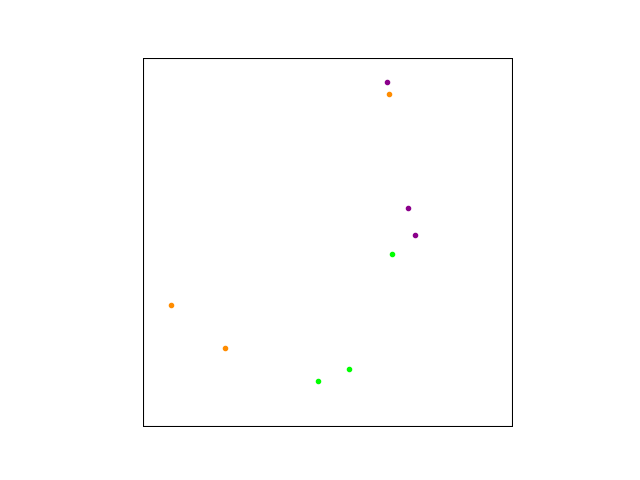
\includegraphics[trim=80 20 80 20,clip, width = .24\textwidth]{chapters/bf/fig/exp_1_instance.png}
    \hspace{-.1in}
    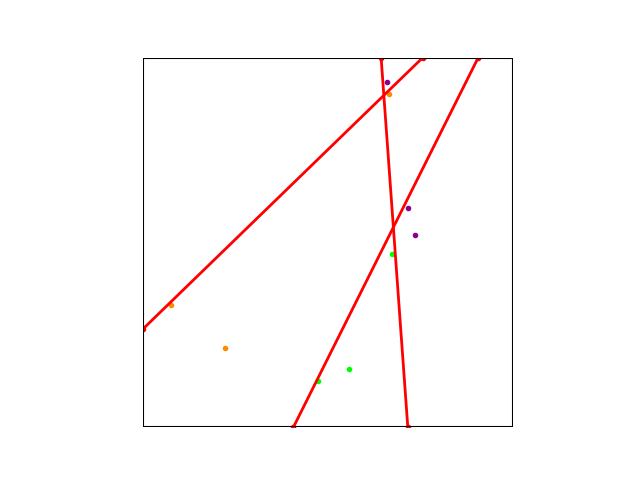
\includegraphics[trim=80 20 80 20,clip, width = .24\textwidth]{chapters/bf/fig/exp_1_result.png}
    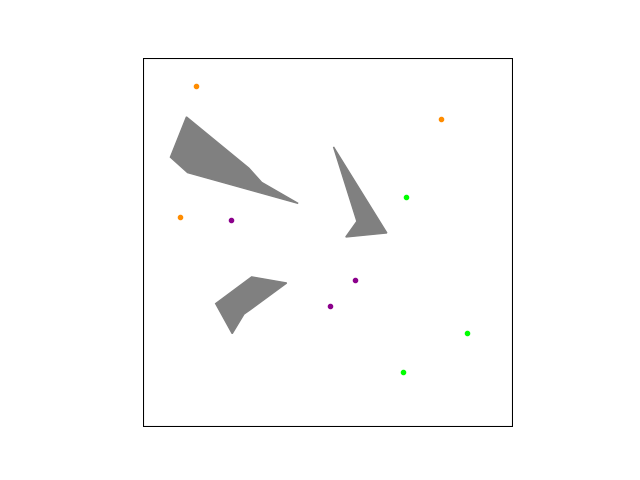
\includegraphics[trim=80 20 80 20,clip, width = .24\textwidth]{chapters/bf/fig/exp_2_instance.png}
    \hspace{-.1in}
    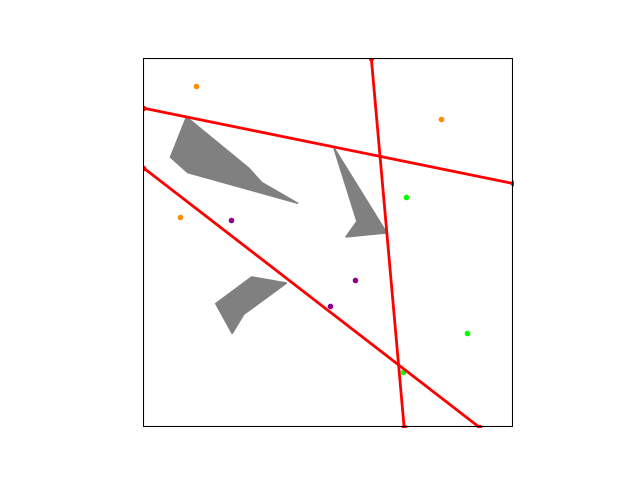
\includegraphics[trim=80 20 80 20,clip, width = .24\textwidth]{chapters/bf/fig/exp_2_result.png}
    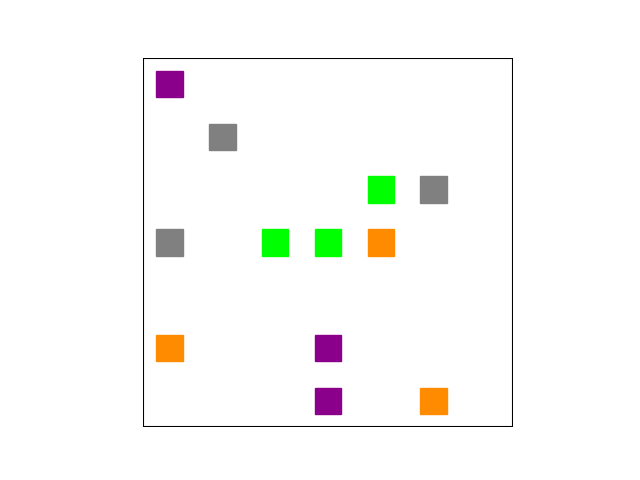
\includegraphics[trim=80 20 80 20,clip, width = .24\textwidth]{chapters/bf/fig/exp_3_instance.png}
    \hspace{-.1in}
    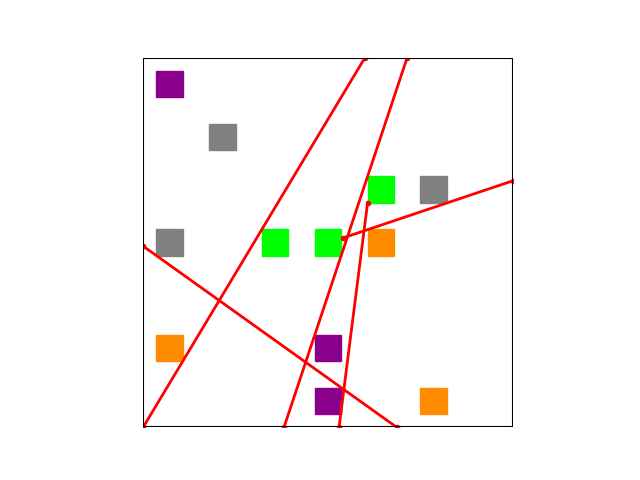
\includegraphics[trim=80 20 80 20,clip, width = .24\textwidth]{chapters/bf/fig/exp_3_result.png}
    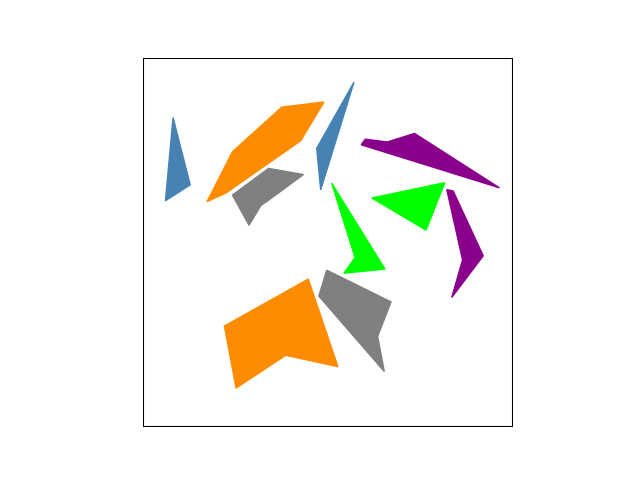
\includegraphics[trim=80 20 80 20,clip, width = .24\textwidth]{chapters/bf/fig/exp_4_instance.png}
    \hspace{-.1in}
    % 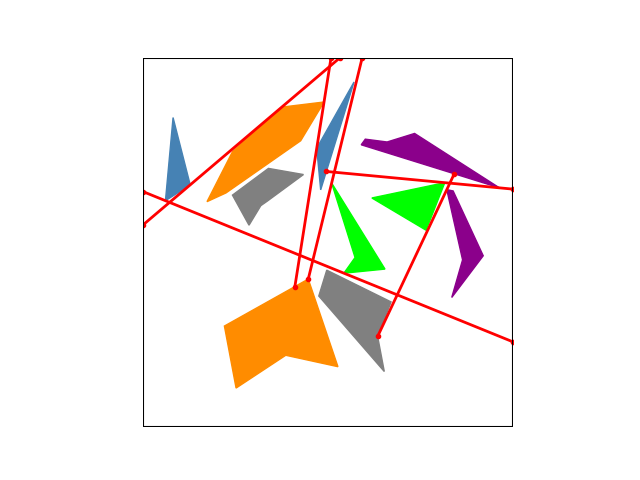
\includegraphics[trim=80 20 80 20,clip, width = .24\textwidth]{fig/exp_4_result.png}
    \begin{overpic}[trim=80 20 80 20,clip, width = .24\textwidth]{chapters/bf/fig/exp_4_result.png}
    \put(-202, 98) {(a)}
    \put(-3, 98) {(b)}
    \put(-202, 0) {(c)}
    \put(-3, 0) {(d)}
    
    \end{overpic}
    \caption{Illustration of the four types of instances used in our  experimental evaluation. (a) Barrier forming for point sets. (b) Barrier forming to separate point sets from polygonal obstacles. (c) Barrier forming to separate uniform square-shaped objects among uniform square-shaped obstacles. (d) Barrier forming to separate random polygonal objects among random polygonal obstacles.}
    \label{fig:bf-exp}
\end{figure*}

\subsection{Separating Sets of Points}
The first type of instances aims at forming barriers among randomly generated point sets, 
shown in ~\ref{fig:bf-exp}(a). The number of object sets to separate from each other range from $2$ to $4$, 
and the number of objects in each set range from $1$ to $6$. 
Each entry in the ~\ref{tab:bf-expr_1} is the result of average computation times over 10 instances. From the result, we observe that the IP based method is fairly effective in separating two sets of objects with the presence of obstacles. The method scales to about $10$ point objects plus obstacles. The number of line segments in the optimal barrier are generally small, e.g., $3$-$10$.

\begin{table}[ht]
    \centering
    \begin{tabular}{|c|c|c|c|c|c|c|}\hline
        %  \diagbox{\#Set}{\#Objects}
        \#Sets &  1 & 2 & 3 & 4& 5& 6\\\hline
 2& 0.005 & 0.011 & 0.083 & 0.419 & 2.010 & 15.887 \\\hline
 3& 0.013 & 0.316 & 12.773 & 962.883 & - & - \\\hline
 4& 0.051 & 14.641 &  -& - &  -&- \\\hline
\end{tabular}
    \caption{Running time in seconds for Expr. 1 where all objects and obstacles are points (~\ref{fig:bf-exp}(a)). ``-'' denotes the result cannot be computed in 1h on average (the same is true for other tables). 
    The column index means the number of objects in each set, and the row index means the number of object sets.
    The number of obstacles is set to be the same as the number of objects for each set. These also apply to the following tables.
    }
    \label{tab:bf-expr_1}
\end{table}

 The second type of instances generates barriers for randomly generated 
 point sets with the existence of polygonal obstacles, shown in ~\ref{fig:bf-exp}(b). 
 The other specification is the same as Expr. 1, and the number of obstacles for each experiment is set to be the same as the number of objects for each set. 
 The resulting time cost, shown in \ref{tab:bf-expr_2}, is similar to Expr. 1 despite the existence of obstacles.
 %
 Similarly, we observe decent performance when it comes to separating two sets of objects among obstacles. 
 %
 The introduction of polygonal obstacles does not cause performance degradation. 


\begin{table}[ht]
    \centering
    \begin{tabular}{|c|c|c|c|c|c|c|}\hline
        %  \diagbox{\#Set}{\#Objects}
        \#Set &  1 & 2 & 3 & 4& 5& 6\\\hline
2& 0.009 & 0.061 & 0.480 & 5.899 & 3.433 & 21.121\\\hline
 3& 0.044 & 3.287 & 71.346 & 320.955 & - & -\\\hline
 4& 0.249 & 13.801 & - & - & - & -\\\hline
    \end{tabular}
    \caption{Running time in seconds for Expr. 2 where objects to be separated are points and obstacles are randomly generated polygons (~\ref{fig:bf-exp}(b)). 
    }
    \label{tab:bf-expr_2}
    \vspace{-2mm}
\end{table}
 
\subsection{Separating Sets of Polygonal Shapes}
The third set of experiments uses randomly placed squares as obstacles and objects, shown in ~\ref{fig:bf-exp}(c). The squares are sampled from a $7\times7$ grid. Each square is half the scale of a grid cell and is positioned at the center of a grid cell. The running time for this case turns out to be the greatest among all $4$ experiments. This is due to the rectlinear nature of the instance, which creates many small cells that are difficult to process. 

\begin{table}[ht]
    \centering
    \begin{tabular}{|c|c|c|c|c|c|c|}\hline
        %  \diagbox{\#Set}{\#Objects}
         \#Set &  1 & 2 & 3 & 4& 5& 6\\\hline
 2 & 0.010 & 0.065 & 0.652 & 31.536 & 575.933 & 1259.653\\\hline
 3 & 0.065 & 10.608 & 337.050 & - & - & -\\\hline
 4 & 0.235 & 124.963 & - & - & - & -\\\hline
    \end{tabular}
    \caption{Running time in seconds for Expr. 3 with square-shaped objects and obstacles (~\ref{fig:bf-exp}(c)). ``-'' denotes the result cannot be computed in 1h on average. 
    % The number of obstacles is set to be the same as the number of objects for each set.
    }
    \label{tab:bf-expr_3}
    \vspace{-2mm}
\end{table}
 
The last type of instances uses random polygons with $3\sim 6$ vertices
as objects and obstacles, shown in ~\ref{fig:bf-exp}(d). 
Counter intuitively, these experiments turn out to have the least time cost among the $4$ experiments despite the most complex environment; we see that even for four different sets of objects where each set contains six objects, the problem can be solved very quickly. %This is due to the larger area of the object sets, which limits the choices of barrier line segments. 

In the end, the running time of the algorithm provided is more dependent on the number of cells and candidate barrier line segments. 
When objects and obstacles are more densely packed in the experiment, 
there will be less barrier candidates and cells due to collisions between objects and the candidate line segments.
While in a sparse environment or even with just point objects, there will be more barrier candidates and cells.
This explains the reduced time cost in a more complex environment from the sparse settings.

\begin{table}[ht]
    \centering
    \begin{tabular}{|c|c|c|c|c|c|c|}\hline
        %  \diagbox{\#Set}{\#Objects}
         \#Set&  1 & 2 & 3 & 4& 5& 6\\\hline
2& 0.006 & 0.031 & 0.080 & 0.143 & 0.157 & 0.156 \\\hline
3& 0.031 & 0.234 & 0.994 & 1.271 & 1.980 & 1.187 \\\hline
4& 0.103 & 0.518 & 3.000 & 6.050 & 9.692 & 17.996 \\\hline 
    \end{tabular}
    \caption{Running time in seconds for Expr. 4 where both the objects to be separated and the obstacles are randomly generated polygons 
    (~\ref{fig:bf-exp}(d)).
    % The number of obstacles is set to be the same as the number of objects for each set.
    }
    \label{tab:bf-expr_4}
    \vspace{-2mm}
\end{table}
